\chapter{Training, Generalization, and Model Selection}
\label{ch:training}

\chapterguide%
  {\chapref{ch:supervised} and \chapref{ch:evaluation}: supervised objectives, realistic holdouts, and metric choice.}
  {diagnose fit, regularize, tune, handle imbalance, select features, and save reproducible models without leakage.}

Training lowers error on the data the model sees; model selection chooses how flexible the model may be without being fooled by noise in the validation set. Every development decision is made before the test set is opened.

\begin{coursechoice}
This chapter sets workflow rules for tuning, feature selection, and imbalance interventions. Chapters 9--14 explain model families; revisit these rules when lasso, trees, and nearest neighbors make them concrete.
\end{coursechoice}

\section{What training is optimizing: empirical risk}

Training commonly minimizes average loss plus a regularization term:
\[
  J(\bm{\theta})
  =\frac{1}{n}\sum_{i=1}^{n}
  \mathcal{L}(y_i,f_{\bm{\theta}}(\bm{x}_i))
  +\lambda\Omega(\bm{\theta}).
\]
The first term fits the observed data; $\Omega$ discourages undesirable complexity. This objective is only a proxy for the true goal of low expected error on future data.

The objective may have one best solution, several equally good ones, or many local dips that can trap an optimizer. Either way, reaching a low training loss does not guarantee good generalization.

\section{Underfitting and overfitting}

\begin{description}[leftmargin=1.15in,style=nextline]
  \item[Underfitting] The model is too simple to capture important patterns and performs poorly even on training data.
  \item[Overfitting] The model learns training-specific noise and performs much worse on unseen data.
  \item[Good fit] The model captures useful patterns and achieves similar, acceptable performance on training and validation data.
\end{description}

\begin{mlfigure}
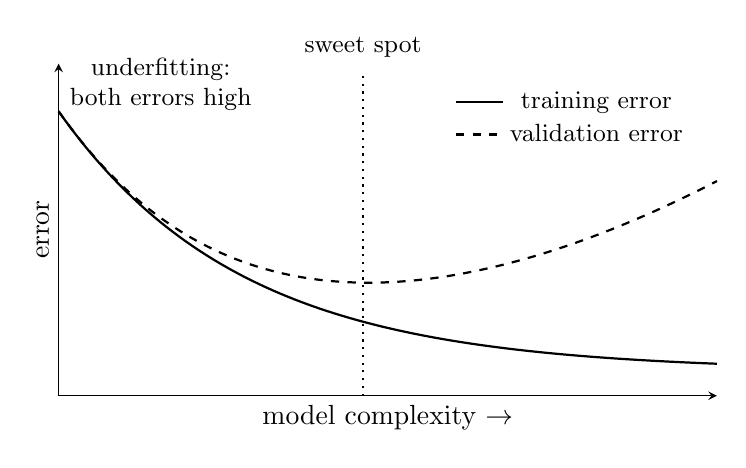
\begin{tikzpicture}
\begin{axis}[
  width=0.82\linewidth, height=5.8cm,
  axis lines=left,
  xlabel={model complexity $\rightarrow$}, ylabel={error},
  ticks=none, domain=0:4, samples=90,
  ymin=0, ymax=1.6, clip=false,
  legend style={draw=none, font=\small, at={(0.97,0.95)}, anchor=north east}
]
\addplot[thick] {1.25*exp(-0.9*x)+0.12};
\addlegendentry{training error}
\addplot[thick, dashed] {1.25*exp(-0.9*x)+0.12+0.055*x^2};
\addlegendentry{validation error}
\draw[dotted, thick] (axis cs:1.85,0) -- (axis cs:1.85,1.55);
\node[font=\small, align=center] at (axis cs:0.62,1.5) {underfitting:\\both errors high};
\node[font=\small, align=center] at (axis cs:3.3,1.32) {overfitting:\\gap grows};
\node[font=\small, align=center] at (axis cs:1.85,1.68) {sweet spot};
\end{axis}
\end{tikzpicture}
\end{mlfigure}

\begin{intuition}
For nested model classes with successful optimization, added flexibility cannot worsen the best training fit. Choose capacity using validation, whose error need not follow a smooth U-curve.
\end{intuition}

% === VISUAL ADDITION: three-fit-regimes ===
\subsection{Underfit, good fit, and overfit on the same observations}

The same observations illustrate three levels of flexibility.

\begin{mlfigure}
\begin{tikzpicture}[baseline=(current bounding box.north)]
\begin{axis}[
  width=0.30\linewidth,height=4.0cm,axis lines=left,ticks=none,
  title={Underfit},title style={font=\small\bfseries\color{MLOrange}},
  xmin=0,xmax=6,ymin=0,ymax=3.2
]
\addplot[only marks,mark=*,mark size=1.6pt,MLBlue] coordinates
  {(0.5,2.5)(1.3,1.45)(2.1,0.82)(3.0,0.58)(3.8,0.82)(4.7,1.45)(5.5,2.55)};
\addplot[MLOrange,very thick,domain=0.3:5.7]{1.45};
\node[font=\scriptsize\color{MLMuted},align=center] at (axis cs:3,2.85) {too simple};
\end{axis}
\end{tikzpicture}
\hfill
\begin{tikzpicture}[baseline=(current bounding box.north)]
\begin{axis}[
  width=0.30\linewidth,height=4.0cm,axis lines=left,ticks=none,
  title={Good fit},title style={font=\small\bfseries\color{MLGreen}},
  xmin=0,xmax=6,ymin=0,ymax=3.2
]
\addplot[only marks,mark=*,mark size=1.6pt,MLBlue] coordinates
  {(0.5,2.5)(1.3,1.45)(2.1,0.82)(3.0,0.58)(3.8,0.82)(4.7,1.45)(5.5,2.55)};
\addplot[MLGreen,very thick,domain=0.3:5.7,samples=80]{0.22*(x-3)^2+0.55};
\node[font=\scriptsize\color{MLMuted},align=center] at (axis cs:3,2.85) {captures the pattern};
\end{axis}
\end{tikzpicture}
\hfill
\begin{tikzpicture}[baseline=(current bounding box.north)]
\begin{axis}[
  width=0.30\linewidth,height=4.0cm,axis lines=left,ticks=none,
  title={Overfit},title style={font=\small\bfseries\color{MLRed}},
  xmin=0,xmax=6,ymin=0,ymax=3.2
]
\addplot[only marks,mark=*,mark size=1.6pt,MLBlue] coordinates
  {(0.5,2.5)(1.3,1.45)(2.1,0.82)(3.0,0.58)(3.8,0.82)(4.7,1.45)(5.5,2.55)};
\addplot[MLRed,very thick,smooth] coordinates
  {(0.3,2.9)(0.5,2.5)(0.9,0.8)(1.3,1.45)(1.7,2.2)(2.1,0.82)
   (2.55,0.25)(3.0,0.58)(3.35,1.7)(3.8,0.82)(4.25,0.3)(4.7,1.45)
   (5.1,2.95)(5.5,2.55)(5.8,1.1)};
\node[font=\scriptsize\color{MLMuted},align=center] at (axis cs:3,2.85) {chases sample noise};
\end{axis}
\end{tikzpicture}
\end{mlfigure}

\begin{keyidea}
Overfitting means following sample-specific noise, not merely fitting a curve.
\end{keyidea}
% === END VISUAL ADDITION ===

\section{Model capacity and the bias-variance trade-off}\label{sec:bias-variance}

Capacity is representational flexibility. Too little may cause bias; too much may increase sensitivity to sampling noise.

For squared-error regression, the expected error at a point $\bm{x}$ decomposes exactly into three parts. Writing $\hat{f}$ for the model trained on a random dataset and $f$ for the true function with noise variance $\sigma^2$,
\[
  \mathbb{E}\!\left[{(y-\hat{f}(\bm{x}))}^2\right]
  =\underbrace{{\left(\mathbb{E}[\hat{f}(\bm{x})]-f(\bm{x})\right)}^2}_{\text{bias}^2}
  +\underbrace{\operatorname{Var}\!\left(\hat{f}(\bm{x})\right)}_{\text{variance}}
  +\underbrace{\sigma^2}_{\text{irreducible noise}}.
\]
Bias is systematic error; variance is sensitivity to training samples; irreducible noise remains. Regularization trades some bias for lower variance.

\begin{workedexample}
At a fixed test point, let $f(\bm{x})=2$ and $\sigma^2=1$. Compare predictions from three model families, each trained on three random datasets.

\begin{mltable}\small
\begin{tabular}{lcccccc}
\toprule
\rowcolor{MLPaleBlue!92}
Model & \multicolumn{3}{c}{Predictions} & $\text{bias}^2$ & Variance & Total \\
\cmidrule(lr){2-4}
 & set 1 & set 2 & set 3 & & & ($+\,\sigma^2=1$) \\
\midrule
Rigid    & $2.6$  & $3.0$ & $3.4$ & $1.000$ & $0.107$ & $\mathbf{2.107}$ \\
Balanced & $1.0$  & $2.0$ & $3.0$ & $0.000$ & $0.667$ & $\mathbf{1.667}$ \\
Wild     & $-1.0$ & $2.0$ & $5.0$ & $0.000$ & $6.000$ & $\mathbf{7.000}$ \\
\bottomrule
\end{tabular}
\end{mltable}

The first row averages $3.0$ against truth $2$, giving bias $1$ and squared bias $1$. Its variance is
\[
  \frac{{(2.6-3)}^2+{(3.0-3)}^2+{(3.4-3)}^2}{3}=\frac{0.16+0+0.16}{3}\approx 0.107,
\]
and the total is $1.000+0.107+1=2.107$.

The rigid model is biased; the wild model is unbiased but highly variable. Minimize total error, not bias alone.

Every row includes irreducible noise $\sigma^2=1$, so no model can reduce expected error below~$1$.
\end{workedexample}

\begin{intuition}
Bias is a tight group of darts away from the bullseye; variance is a wide scatter around it. Irreducible noise is a wobbling dartboard.
\end{intuition}

More data often reduces variance; stronger assumptions may exchange bias for lower variance. Choose reliable validation performance over complexity.

\section{Regularization}

Regularization discourages unnecessarily large or complex parameter values. Two common penalties are
\[
  J_{L_1}(\bm{\theta})=J(\bm{\theta})
  +\lambda\sum_{j=1}^{p}|\theta_j|,
\]
\[
  J_{L_2}(\bm{\theta})=J(\bm{\theta})
  +\lambda\sum_{j=1}^{p}\theta_j^2.
\]
$L_1$ regularization can make some parameters exactly zero. $L_2$ regularization smoothly shrinks large parameters. The strength $\lambda$ is normally selected with validation data.

\begin{workedexample}
For the one-parameter objective $\tfrac12(\beta-\hat\beta_{\text{OLS}})^2$ with $\hat\beta_{\text{OLS}}=4$, ridge adds $\lambda\beta^2/2$ and lasso adds $\lambda|\beta|$. Their solutions are
\[
  \hat{\beta}_{\text{ridge}}=\frac{\hat{\beta}_{\text{OLS}}}{1+\lambda},
  \qquad
  \hat{\beta}_{\text{lasso}}=\operatorname{sign}(\hat{\beta}_{\text{OLS}})\max\!\left(|\hat{\beta}_{\text{OLS}}|-\lambda,\;0\right).
\]

\begin{mltable}\small
\begin{tabular}{cccl}
\toprule
\rowcolor{MLPaleBlue!92}
$\lambda$ & Ridge & Lasso & What happened \\
\midrule
$0$ & $4.000$ & $4.000$ & no penalty; both give the OLS answer \\
$1$ & $2.000$ & $3.000$ & ridge halves it; lasso subtracts a flat $1$ \\
$5$ & $0.667$ & $0.000$ & ridge is small but alive; lasso has deleted the feature \\
\bottomrule
\end{tabular}
\end{mltable}

Here ridge divides by $1+\lambda$, approaching zero without reaching it at finite $\lambda$. Lasso subtracts $\lambda$ and clips at zero once $\lambda\ge4$.
\end{workedexample}

\subsection{Other ways to regularize}

Regularization is broader than adding a penalty to the objective.

\begin{itemize}
  \item \term{Early stopping} retains the model from the epoch with the best validation performance.
  \item \term{Data augmentation} adds meaningful input variation without changing labels.
    \item \term{Pruning} removes weak branches, features, or parameters.
  \item \term{Ensembling} averages several models to reduce variance.
  \item \term{Noise injection} trains the model to remain stable under small perturbations.
\end{itemize}

Match regularization to the failure mode; it cannot fix leakage or distribution mismatch.

\section{Learning curves}

A learning curve plots training and validation performance against training-set size or training time.

\begin{itemize}
  \item Poor training and validation performance suggests underfitting or an optimization problem.
  \item Strong training performance with weak validation performance suggests overfitting.
  \item Improvement in both curves as more data is added suggests that additional representative data may help.
  \item Highly unstable curves suggest sensitivity to the split, seed, or a small validation sample.
\end{itemize}

\subsection{Reading learning curves in practice}

\begin{mlfigure}
\begin{tikzpicture}[baseline=(current bounding box.north)]
\begin{axis}[
  width=0.46\linewidth, height=4.3cm, axis lines=left,
  title style={font=\small\bfseries\color{MLRed}}, title={High variance (overfitting)},
  xlabel={Training rows}, ylabel={Error},
  label style={font=\scriptsize\color{MLMuted}}, tick label style={font=\scriptsize\color{MLMuted}},
  legend style={font=\scriptsize,draw=none,fill=none,at={(0.98,0.96)},anchor=north east},
  xmin=0, xmax=1000, ymin=0, ymax=0.5
]
\addplot[MLBlue,very thick,mark=*,mark size=1.2pt] coordinates
  {(50,0.01)(150,0.02)(300,0.03)(600,0.04)(1000,0.05)}; \addlegendentry{train}
\addplot[MLRed,very thick,mark=square*,mark size=1.2pt] coordinates
  {(50,0.45)(150,0.36)(300,0.31)(600,0.27)(1000,0.25)}; \addlegendentry{validation}
\end{axis}
\end{tikzpicture}
\hfill
\begin{tikzpicture}[baseline=(current bounding box.north)]
\begin{axis}[
  width=0.46\linewidth, height=4.3cm, axis lines=left,
  title style={font=\small\bfseries\color{MLOrange}}, title={High bias (underfitting)},
  xlabel={Training rows}, ylabel={Error},
  label style={font=\scriptsize\color{MLMuted}}, tick label style={font=\scriptsize\color{MLMuted}},
  legend style={font=\scriptsize,draw=none,fill=none,at={(0.98,0.96)},anchor=north east},
  xmin=0, xmax=1000, ymin=0, ymax=0.5
]
\addplot[MLBlue,very thick,mark=*,mark size=1.2pt] coordinates
  {(50,0.20)(150,0.24)(300,0.26)(600,0.27)(1000,0.28)}; \addlegendentry{train}
\addplot[MLRed,very thick,mark=square*,mark size=1.2pt] coordinates
  {(50,0.38)(150,0.33)(300,0.31)(600,0.30)(1000,0.30)}; \addlegendentry{validation}
\end{axis}
\end{tikzpicture}
\end{mlfigure}

\begin{keyidea}
A persistent gap suggests variance: try more representative data or stronger regularization. Both curves poor suggest limited signal, underfitting, or optimization failure; investigate features and fitting.
\end{keyidea}

\section{Hyperparameter tuning}
\label{sec:hyperparameter-tuning}

Hyperparameters include regularization strength, tree depth, number of neighbors, learning rate, and model size. Common search methods are:

\begin{mltable}
\begin{tabularx}{\linewidth}{@{}>{\bfseries\leavevmode\color{MLNavy}}p{0.22\linewidth}p{0.39\linewidth}X@{}}
\toprule
\rowcolor{MLPaleBlue!92}
Method & Search strategy & Main consideration \\
\midrule
Grid search & Evaluates every combination in a fixed Cartesian grid. & Becomes expensive as the number of dimensions and candidate values grows. \\
Random search & Samples combinations from the search space. & Often explores high-dimensional spaces more efficiently. \\
Sequential search & Uses earlier results to choose promising later experiments. & Concentrates the search on regions that appear useful. \\
\bottomrule
\end{tabularx}
\end{mltable}

Use identical validation across candidates. Repeated tuning can overfit validation, so retain an untouched final test set.

\subsection{Tuning without fooling yourself}

\begin{intuition}
Random search explores more distinct values when few hyperparameters matter. Small grids suit one or two controls; neither fixes invalid validation.
\end{intuition}

\subsection{Nested cross-validation for the selection procedure}

Tune inside each outer training split; outer holdouts evaluate the complete search-plus-model procedure. Lab~2, Part~D instead uses one training-only search and a final test.

\section{Imbalanced classification: change the policy, not the test set}

Imbalance can make majority predictions look accurate while missing rare cases. Consider metrics, thresholds, class weights, and training-only resampling.

\begin{mltable}
\begin{tabularx}{\linewidth}{@{}>{\bfseries\leavevmode\color{MLNavy}}p{0.24\linewidth}X@{}}
\toprule
\rowcolor{MLPaleBlue!92}
Strategy & How it helps \\
\midrule
Change the metric first & For rare-class performance, use recall, precision, balanced accuracy, or average precision rather than accuracy alone (\chapref{ch:evaluation}). \\
Move the threshold & Choose a lower probability cutoff on validation data to increase recall without retraining. \\
Class weights & Tell the model that a mistake on the rare class costs more (\texttt{class\_weight="balanced"}). Lab~2's grid search includes this option and selects it. \\
Resampling & Drop majority rows (\term{undersampling}) or add minority examples (\term{oversampling}). SMOTE interpolates between nearby minority examples. Resample only within each validation split\textquotesingle s training portion. \\
\bottomrule
\end{tabularx}
\end{mltable}

\begin{coursechoice}
SMOTE's geometry is developed in \chapref{ch:knn-nb}. Its rule applies now: split first and synthesize only within training folds, never from held-out observations.
\end{coursechoice}

\begin{pitfall}
Resampling changes training prevalence, not the target evaluation population. Keep validation and test distributions realistic.
\end{pitfall}

\section{Feature selection is part of model development} \label{sec:feature-selection}

\term{Feature selection} keeps a subset of the original columns to cut cost, noise, or complexity. It is not always worth doing: a regularized model with a modest number of features may not need it.

Selection retains original columns; extraction creates new ones, as in PCA (\chapref{ch:dimred}).

\begin{mltable}
\begin{tabularx}{\linewidth}{@{}>{\bfseries\leavevmode\color{MLNavy}}p{0.19\linewidth}p{0.38\linewidth}X@{}}
\toprule
\rowcolor{MLPaleBlue!92}
Family & How it works & Main trade-off \\
\midrule
Filter methods & Score features by variance, correlation, tests, or mutual information before model fitting. & Fast and model-agnostic, but may miss interactions. \\
Wrapper methods & Fit a model on different feature subsets, as in recursive feature elimination. & Model-specific, but computationally expensive. \\
Embedded methods & Use selection learned during fitting: zero lasso coefficients or tree-based importances. & Efficient, but inherits model assumptions and instability. \\
\bottomrule
\end{tabularx}
\end{mltable}

\begin{secondpass}
Revisit lasso in \chapref{ch:regression}, tree importances in \chapsref{ch:decision-trees}{ch:ensembles}, and irrelevant dimensions in \chapref{ch:knn-nb}. The validation rules stay the same.
\end{secondpass}

\begin{pitfall}
Fit supervised selectors inside the validated pipeline, separately in each training fold. Selecting once on all labels leaks information; the number of retained features is also a hyperparameter.
\end{pitfall}

\begin{keyidea}
Before selecting features, specify the goal: accuracy, collection cost, or interpretability. Validate selection together with the model, without using the test set.
\end{keyidea}

\begin{debugtask}
A researcher selects the top 20 features using all labeled rows, applies SMOTE to the full table, then runs cross-validation and reports the best result. Redesign the experiment so that nothing from the held-out rows can influence selection, resampling, or tuning.
\end{debugtask}

\section{Reproducible training}

A reproducible experiment records:

\begin{itemize}
  \item data and preprocessing versions;
  \item training, validation, and test identifiers;
  \item software and hardware environment;
  \item model specification and configuration;
  \item hyperparameters, random seeds, and stopping rules;
  \item training curves, checkpoints, and evaluation outputs.
\end{itemize}

Report variation across reruns rather than one favorable seed; parallel hardware may prevent bit-for-bit reproduction.

\begin{keyidea}
Training fit and generalization are distinct requirements.
\end{keyidea}

\begin{modelcard}{Training and Tuning - Practical Checklist}
\begin{tabularx}{\linewidth}{@{}>{\bfseries\leavevmode\color{MLNavy}}p{0.24\linewidth}X@{}}
Objective & Define the training objective and know which parts are learned from data; optimizer details are second-pass when the estimator exposes them. \cr
Diagnosis & Compare training and validation curves to identify underfitting or overfitting. \cr
Regularization & Limit model capacity with penalties, pruning, simpler features, or early stopping. \cr
Tuning & Search hyperparameters using validation data or nested cross-validation, not the final test set. \cr
Reproducibility & Record the data version, split logic, preprocessing, model specification, random seeds, software versions, and hardware-relevant settings. \cr
\end{tabularx}
\end{modelcard}

\subsection{A short reproducibility checklist}

\begin{mltable}
\begin{tabularx}{\linewidth}{@{}>{\bfseries\leavevmode\color{MLNavy}}p{0.05\linewidth}X@{}}
\toprule
\rowcolor{MLPaleBlue!92}
\normalfont\bfseries\leavevmode\color{MLNavy}\checkmark & \normalfont\bfseries\leavevmode\color{MLNavy}Record this before you call a model finished \\
\midrule
1 & The exact data snapshot, with a date and a row count. \\
2 & Every random seed used. \\
3 & Library versions. \\
4 & The complete preprocessing and modeling procedure, not only the final estimator. \\
5 & The chosen hyperparameters and the search space they came from. \\
6 & The metric, the split strategy, and the final test score. \\
7 & Known limitations: who the model is likely to be wrong about. \\
\bottomrule
\end{tabularx}
\end{mltable}

\begin{keyidea}
Record weakly represented populations and known subgroup failures. These limits guide responsible use, not a judgment that the project failed.
\end{keyidea}

\subsection{Save the model you would deploy}

After locking and testing the procedure, save the whole preprocessing-and-estimator pipeline with a model card for reuse.

\begin{lstlisting}[style=mlpython]
import joblib, json

joblib.dump(final_model, MODELS / "titanic_survival.joblib")
(MODELS / "titanic_survival_card.json").write_text(json.dumps({
    "features": features,                 # the columns the model expects
    "final_test_roc_auc": 0.837,          # the one test result
    "decision_threshold": 0.5,            # the policy chosen on validation data
    "scikit_learn_version": sklearn.__version__,
}, indent=2))

loaded = joblib.load(MODELS / "titanic_survival.joblib")
loaded.predict_proba(new_rows)            # new_rows has the same columns as training
\end{lstlisting}

Verify the saved artifact:

\begin{itemize}
  \item \textbf{Save the pipeline.} Include fitted scaling and encoding, not just the estimator.
  \item \textbf{Check that the file reproduces the test predictions.} Load it back and compare with the in-memory model before calling it done.
  \item \textbf{Include a model card:} features, threshold, test score, and library version. Lab~2 saves the model; Lab~3 verifies it; \texttt{predict\_passenger.py} loads it.
\end{itemize}

\begin{tryit}
Repeat training and validation across prespecified seeds and splits. Report variation, lock the seed policy and model, refit, then test once.
\end{tryit}

\begin{debugtask}
A hyperparameter search reports its best configuration, then the researcher reruns the search with a narrower grid chosen after inspecting the test score. Explain how the test set entered training decisions and redesign the selection/final-evaluation boundary.
\end{debugtask}

\begin{decisionmemo}
Two models have nearly equal mean validation performance. One has lower fold-to-fold variation, half the inference latency, and simpler monitoring. Decide which to keep and state why a tiny mean-score advantage is not automatically decisive.
\end{decisionmemo}

\begin{tryit}
Using fixed validation folds, compare training and validation performance across capacities. Tune on development data, lock the procedure, and list the refitting steps before one final test.
\end{tryit}

\begin{quickcheck}
\begin{enumerate}
  \item What train-versus-validation pattern suggests underfitting, and what pattern suggests overfitting?
  \item How can regularization improve validation performance even while making the training fit worse?
  \item Which decisions must be locked before the final test set is evaluated?
\end{enumerate}
\end{quickcheck}
